% How to use writeLaTeX: 
%
% You edit the source code here on the left, and the preview on the
% right shows you the result within a few seconds.
%
% Bookmark this page and share the URL with your co-authors. They can
% edit at the same time!
%
% You can upload figures, bibliographies, custom classes and
% styles using the files menu.
%
%%%%%%%%%%%%%%%%%%%%%%%%%%%%%%%%%%%%%%%%%%%%%%%%%%%%%%%%%%%%%%%%%%%%%%

\documentclass[12pt,english,brazil]{article}
\usepackage{sbc-template}
\usepackage{adjustbox}
\usepackage{graphicx,url}
\usepackage{graphics}
\usepackage{color}
\usepackage{colortbl}
\usepackage[utf8]{inputenc}  
% Coloquei esse pacote para tamanho pequeno de fonte
\usepackage{scalefnt}
\usepackage{multirow}
\usepackage{subfigure}
\usepackage{multicol}
\usepackage{babel}
\babeltags{br = brazil, en = english}
\usepackage[T1]{fontenc}
\usepackage{xspace}
\usepackage{url}

\usepackage{xargs}
\usepackage[colorinlistoftodos,prependcaption,textsize=tiny]{todonotes}
\newcommandx{\ups}[2][1=]{\todo[linecolor=red,backgroundcolor=red!25,bordercolor=red,#1]{\tiny Gerson: #2}\xspace}
\newcommandx{\aham}[2][1=]{\todo[linecolor=yellow,backgroundcolor=yellow!25,bordercolor=yellow,#1]{\tiny Gui: #2}\xspace}
     
\sloppy

\title{Estudo de viabilidade do uso de Raspberry como servidor R-Shiny}

\author{Guilherme de Souza\inst{1}}


\address{Programa de Pós-Graduação em Computação \\Universidade Federal de Pelotas (UFPel)\\
  Caixa Postal 354 -- 96010.610 -- Pelotas -- RS -- Brazil
\nextinstitute
  Instituto de Matemática e Estatística (IME) -- Universidade de São Paulo (USP)\\
  Rua do Matão, 1010 -- São Paulo -- SP -- Brazil
  \email{\{gdsdsilva,gerson.cavalheiro\}@inf.ufpel.edu.br, gold@ime.usp.br}
}

\begin{document} 

\maketitle
    
\en
\begin{abstract}


\end{abstract}

\br
\begin{resumo} 


\end{resumo}



\section{Introdução}

A decisão economica sobre diferentes frentes por vezes passa pela análise de uma grande massa de dados. R é uma ferramenta que oferece grande potencial para manipulação e visualização de massas de dados. Shiny é um pacote para R que permite que servidores disponibilizem recursos para visualizações R.

R é uma ferramenta livre, existem outras, X e Y, que oferecem soluções semelhantes, porém, em um contexto proprietário. Este trabalho tem por objetivo avaliar o poder de escalabilidade de servidores web R, utilizando shiny.

O caso de estudo encaminhado considera o serviço WebShyda. São consideradas duas plataformas de suporte: um servidor com arquitetura convencional e um dispositivo de baixa capacidade (small board). O objetivo deste estudo é identificar componentes do sw, atualmente construído de forma monolítica, em microserviços. 

\section{Trabalhos Relacionados} \label{sec:TrabalhosRelacionados}

\section{WebSyhda}\label{sec:websyhda}
Engenharia e gestão de recursos hídricos mantém uma grande dependência de séries hidrológicas. No entanto, o processamento destas séries é complexo, geralmente dependente de métodos numéricos para resolução, e é suscetível a erros quando feito de forma manualmente. Esses aspectos frequentemente dificultam a elaboração de projetos que depende da análise e estudo de séries hidrológicas. Com isso O Grupo de Pesquisa em Hidrologia e Modelagem Hidrológica em Bacias Hidrográficas/CNPq da UFPEL, propôs, desenvolveu e mantem O \emph{System of Hydrological Data Acquisition and Analysis} ou SYHDA \cite{syhda}.

A plataforma recentemente passou por uma migração para o modelo Web, onde encontra-se em constante desenvolvimento. É integralmente desenvolvida em R, com auxílio do RStudio e de inúmeras bibliotecas gratuitas de uso geral, uso específico para a hidrologia e de funcionalidades para ambiente Web. %li no cobalto

O WebSYHDA permite a importação de dados do Hidroweb/ANA\footnote{ANA: \url{https://dadosabertos.ana.gov.br}}, para dados de vazão, chuva e nível. Estes dados são reconhecidos pela plataforma de forma automática. Outras fontes de dados estão sendo implementadas na plataforma, como BDMEP/INMET\footnote{INMET: \url{https://portal.inmet.gov.br}} e dados oriundos de estações de monitoramento diversas com formatos definidos pelo usuário.

A plataforma em sua versão atual, conta com diversas funcionalidades, bem como: estatísticas descritivas, representações gráficas, testes não paramétricos, análises de sazonalidade, consistência de dados de chuva, curvas IDF, análise de frequência local e análise de frequência regional. Os resultados serão estruturados de forma dinâmica, assim permitindo o manuseio pelo usuário final, permitindo ainda a possibilidade de exportação e salvar o estado atual do projeto. 

\section{Metodologia} \label{sec:metodologia}

Visto que a demanda de serviços \textit{web} ocupa a maior parte das aplicações na nuvem, j

para a realização deste trabalho optou-se pelo uso de um banco de dados NoSQL, dada sua adequação ao uso em sistemas distribuídos e em aplicações com alta demanda e dependentes de elasticidade \cite{cattell2011scalable}. Tendo tudo isso em vista, optamos por fazer uso do banco de dados NoSQL Apache Cassandra.

Da mesma forma, para escolha do simulador entre os \textit{benchmarks} disponíveis para testes em sistemas de nuvem, optou-se pelo que seria capaz de atender nossas exigências de latência e que nos permitisse uma livre escolha das cargas de trabalho para criarmos cenários restritos para execução dos experimentos com cargas ideais e próximas à capacidade de processamento da Raspberry. Dadas tais necessidades, entre outras funções, o simulador \textit{NDBench} foi o selecionado para o presente trabalho. 



\subsection{Linguagem R} \label{sec:R}

R é uma linguagem e ambiente com foco em computação estatística e gráficos. Assim, R permite desenvolver e publicar gráficos bem projetados \cite{whatR}, semelhantemente a C/C++ e outras disponíveis no mercado R também permite o desenvolvimento por meio de módulos, mas ainda se tratando de um unico e grande serviço.
%Colocar sobre a forma de escalabilidade do R aqui?!

Com isso vale ressaltar que R é uma aplicação de thread único, o que significa que um aplicativo não pode atender a dois usuários diferentes precisamente ao mesmo tempo, Figura ~\ref{singleThreads}. Em muitas aplicações isso não é um problema, porque a maioria dos cálculos leva apenas dezenas ou centenas de milissegundos. Como resultado, um único processo R geralmente pode atender de 5 a 30 solicitações / segundo \cite{ShinyappsEscalabilidade}. 

\begin{figure}[htbp]
  \centering 
  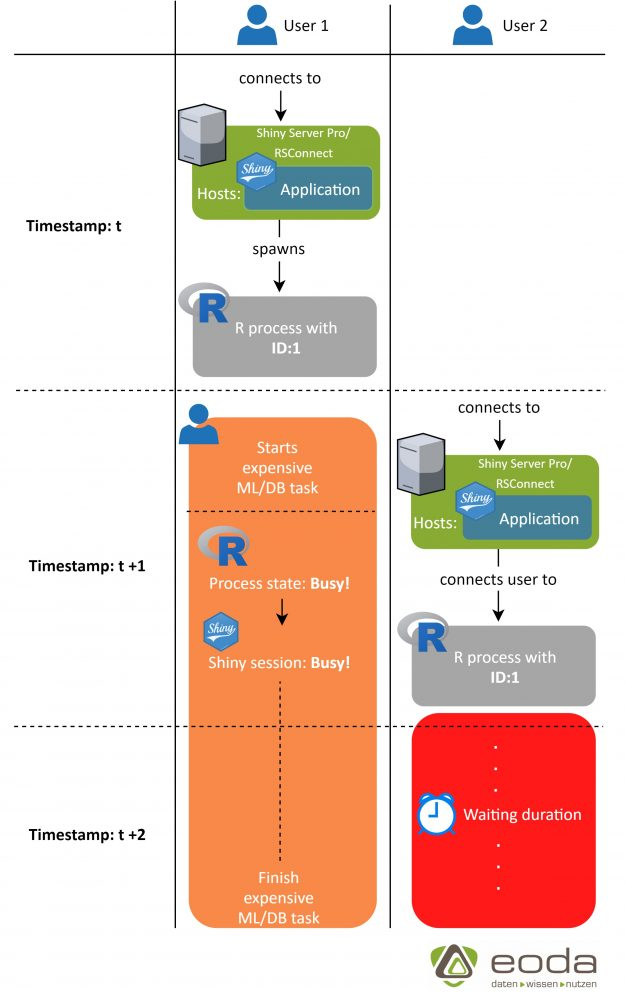
\includegraphics[scale=.5]{figures/single_threads.jpg}
  \caption{Exemplo de uma execução sequencial \cite{singleThreads}}
  \label{singleThreads}
\end{figure}

\subsection{Shiny} \label{sec:Shiny}

Para o desenvolvimento de aplicativos \emph{web} fazendo uso da linguagem R, a Rstudio mantém o pacote \emph{Shiny}\footnote{Shiny: \url{https://shiny.rstudio.com}}. Um pacote R que facilita a construção de aplicativos interativos. Permitindo hospedar aplicativos independentes em uma página da web ou incorporá-los em documentos R Markdown ou construir painéis. Permitindo ainda, estender os aplicativos \emph{Shiny} com temas CSS (\emph{Cascading Style Sheets}), \emph{htmlwidgets} e ações JS (\emph{JavaScript}).

\subsection{Shinycannon} \label{sec:Shinycannon}

\textit{Shinycannon}\footnote{Shinycannon: \url{https://github.com/rstudio/shinycannon}} é uma ferramenta de linha de comando que possibilita testes de carga em aplicativos R. De forma a permitir aos desenvolvedores analisarem a escalabilidade de seu aplicativo simulando de um a n usuários simultaneos.

A Ferramenta acompanha o pacote \textit{shinyloadtest}\footnote{Shinyloadtest: \url{https://rstudio.github.io/shinyloadtest/}}, mantido pela própria Rstudio. O pacote é responsavel por gerar uma gravação de uma sessão de usuário, essas sessões podem ser criadas pensando no uso tipico do aplicativo desenvolvido\cite{shinyloadtest}. A sessão é criada de forma manual, após a iniciação do pacote o tester executa a interação com o aplicativo de forma natual, assim como um usuário comum. Ao terminar seu uso basta fechar a aplicação para que o pacote encerre a gravação da sessão.

Com isso, por sua vez, a \textit{Shinycannon} permite a criação de trabalhadores, que são os usuários simulados, podendo criar tantos quantos necessarios para execução dos testes. Assim para execução dos teste devemos definir o numero de trablhadores e o tempo total da sessão que será executada pelos mesmos. 

Em suma, a \textit{Shinycannon} replica os passos da gravação criada pelo pacote \textit{Shinyloadtest} entre seus trabalhadores (usuários), fazendo com que cada trabalhador execute simultaneamente a mesma sessão durante o tempo definido pelo desenvolvedor.

\subsection{Metodologia dos Testes}\label{sec:MetodologiaDosTestes}

Todo o roteiro de testes e os arquivos necessários aqui apresentados estão disponíveis no GitHub\footnote{GitHub: \url{https://github.com/SouzaGuilherme/research_PI3_R-Shiny-server}}.

\section{Resultados} \label{sec:Resultados}


\section{Conclusão} \label{sec:conlusao}



\bibliographystyle{sbc}
\bibliography{sbc-template}

\end{document}
